\section{Results}
\label{sec:results}

This section reports the results of the conducted experiments. The model architectures, the
training procedure and the construction of the frozen feature extractor are
described in detail in the methodology, so here we recall only what is needed to
read the figures and tables.

\subsection{Experiment 3: Quantum and Classical Heads on Frozen Features}
\label{sec:exp3}

Coming from the prior experiments, where we found no advantage for quantum models
over classical solutions, we push the problem harder and ask whether a quantum head
can be more parameter-efficient than a classical one on a hard four-class spectral
task. The four classes are \texttt{STAR\_BROWN\_DWARF\_L}, \texttt{STAR\_M8},
\texttt{GALAXY\_STARBURST} and \texttt{GALAXY\_STARFORMING}, balanced to 1000 samples
per class and split $70/15/15$ into train, validation and test. As detailed in
Section~\ref{sec:exp3_methods}, every head sits on the same frozen feature extractor
and receives the same 128-dimensional feature vector, so any difference comes from
the head alone. The four heads are the dense classical baseline (Model~A, 5058
parameters), the hybrid quantum head (Model~B, 556 parameters) and two
parameter-matched classical controls with a ReLU or a $\tanh$ middle stage
(Models~C and~D, 556 parameters each). Models~C and~D share the exact shape and
parameter count of Model~B, so the comparison isolates the quantum circuit rather
than the surrounding structure.

\subsubsection{Overall classification performance}

Table~\ref{tab:exp3_headline} summarises the headline results and
Figure~\ref{fig:exp3_cm} shows the corresponding test confusion matrices. The dense
classical head (A), the quantum head (B) and the Tanh control (D) all reach roughly
96\% overall accuracy with very similar per-class behaviour, while the ReLU control
(C) collapses to about 79\%. The three successful models classify the hardest
class, \texttt{STAR\_BROWN\_DWARF\_L}, with recall between 0.93 and 0.95 and confuse
it almost only with \texttt{STAR\_M8}, the spectrally adjacent class. Notably the
556-parameter quantum head (B) and the 556-parameter Tanh control (D) match the
$9\times$ larger 5058-parameter dense head (A) at the same accuracy, which shows
that a tiny head is sufficient once the features are supplied by a strong frozen
extractor.

\begin{table}[t]
\centering
\caption{Experiment 3 headline results on the four-class test set. Accuracies are
read from the confusion matrices and should be treated as $\pm 1$ percentage point.
BD recall is the recall on the brown-dwarf class \texttt{STAR\_BROWN\_DWARF\_L}.}
\label{tab:exp3_headline}
\setlength{\tabcolsep}{4pt}
\footnotesize
\begin{tabular}{llccc}
\toprule
 & Head & Params & Acc. & BD recall \\
\midrule
A & Dense classical    & 5058 & $\sim$96\% & 0.95 \\
B & Quantum (Lin.+VQC) & 556  & $\sim$96\% & 0.93 \\
C & Classical, ReLU    & 556  & $\sim$79\% & 0.18 \\
D & Classical, Tanh    & 556  & $\sim$96\% & 0.94 \\
\bottomrule
\end{tabular}
\end{table}

\begin{figure*}[t]
\centering
\begin{subfigure}{0.45\textwidth}
  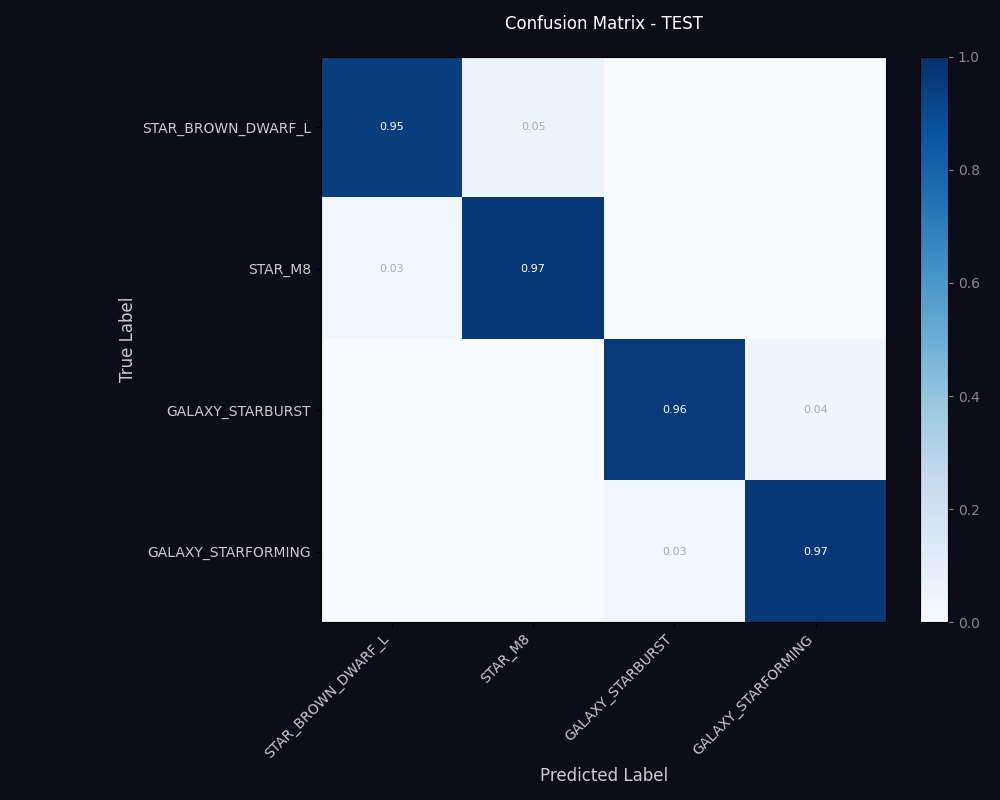
\includegraphics[width=\linewidth]{Figures/5000param_classical_cm_test.png}
  \caption{Dense classical, 5058 params (A).}
  \label{fig:exp3_cm_dense}
\end{subfigure}\hfill
\begin{subfigure}{0.45\textwidth}
  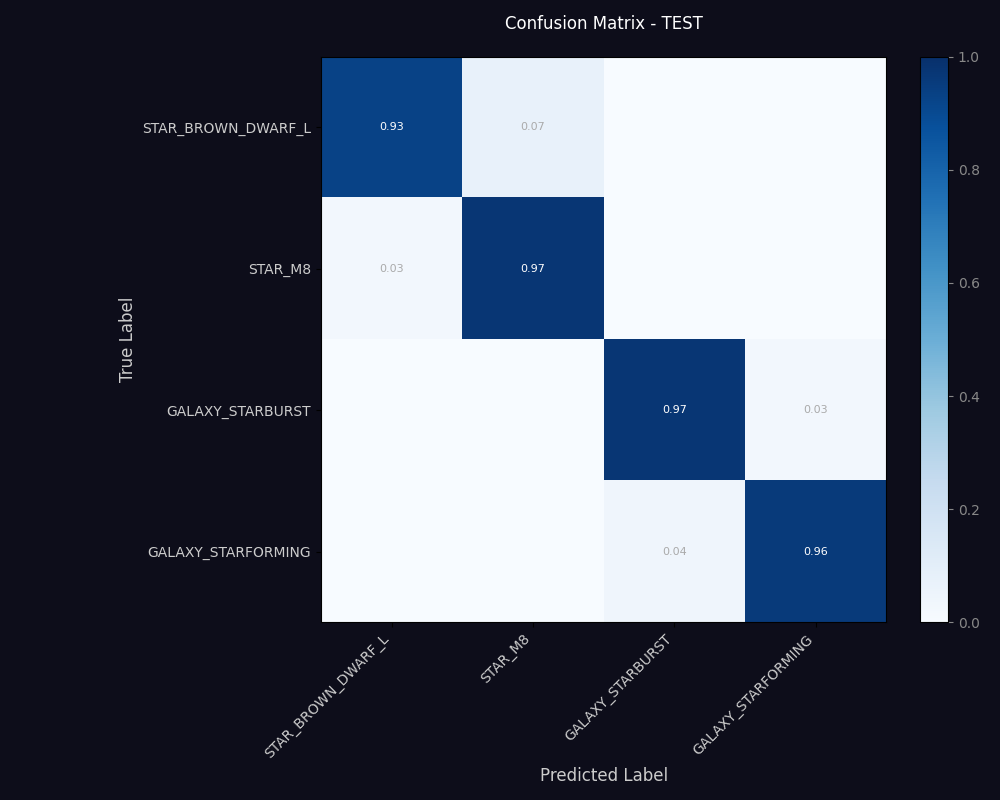
\includegraphics[width=\linewidth]{Figures/quantum_500param_cm_test.png}
  \caption{Quantum, 556 params (B).}
  \label{fig:exp3_cm_quantum}
\end{subfigure}

\vspace{0.5em}

\begin{subfigure}{0.45\textwidth}
  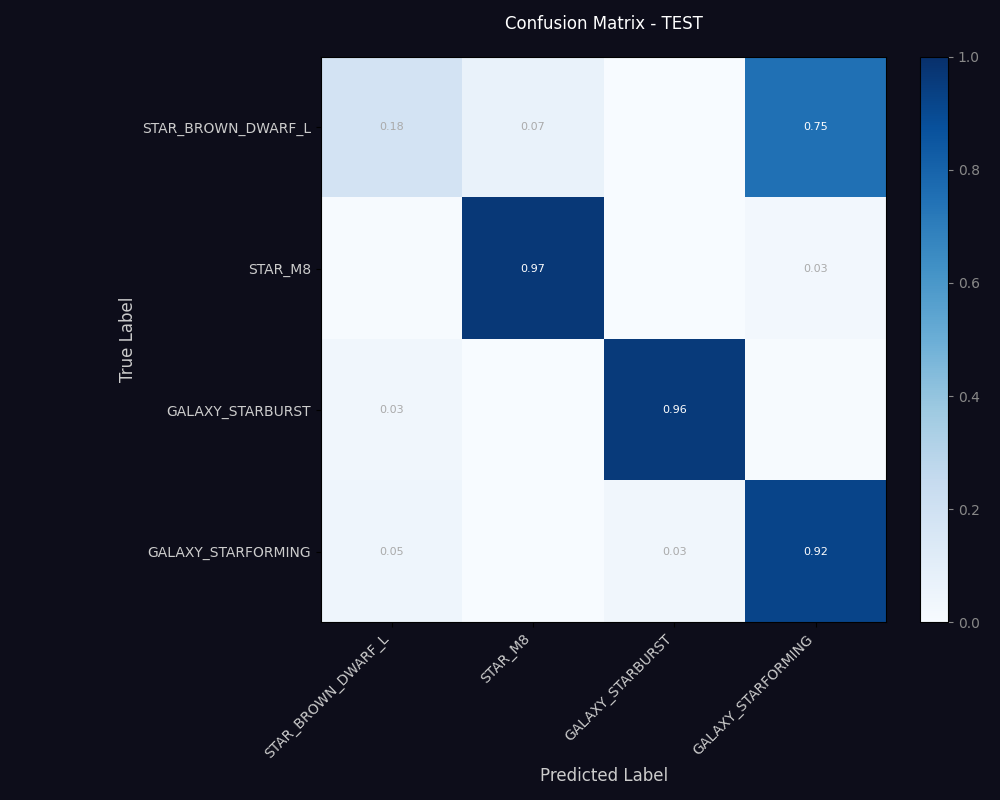
\includegraphics[width=\linewidth]{Figures/500param_classical_deadrelu_cm_test.png}
  \caption{Classical ReLU control, 556 params (C).}
  \label{fig:exp3_cm_relu}
\end{subfigure}\hfill
\begin{subfigure}{0.45\textwidth}
  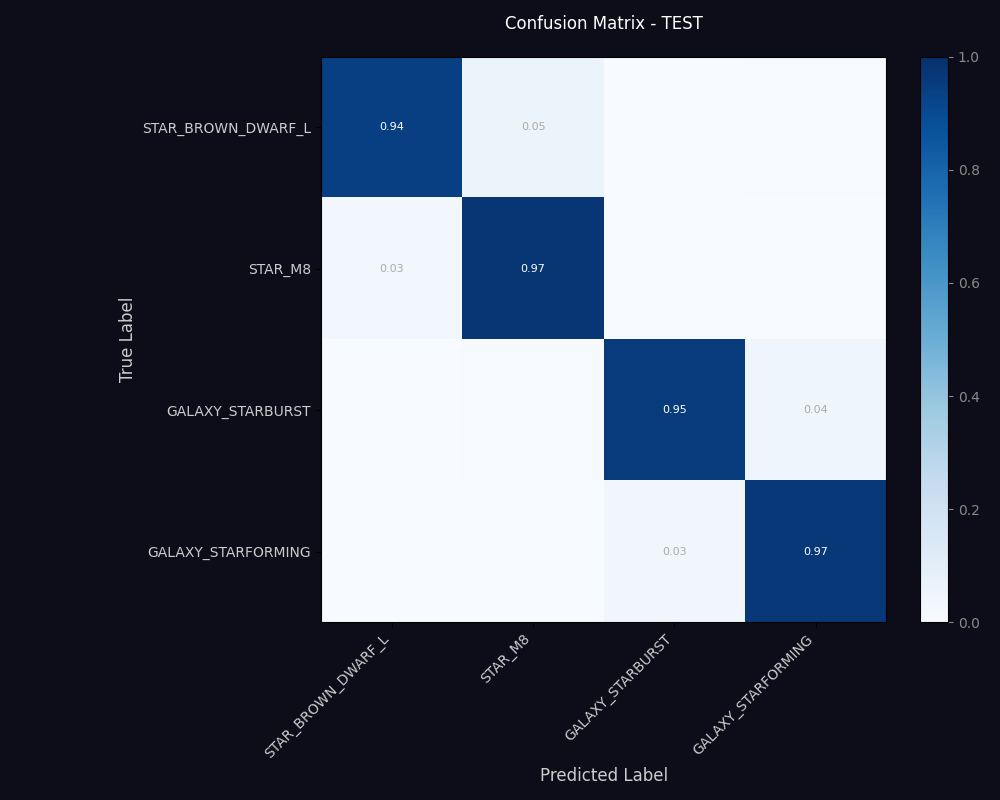
\includegraphics[width=\linewidth]{Figures/500param_classical_tanh_cm_test.png}
  \caption{Classical Tanh control, 556 params (D).}
  \label{fig:exp3_cm_tanh}
\end{subfigure}
\caption{Test-set confusion matrices for the four heads. The dense head (A), the
quantum head (B) and the Tanh control (D) are almost indistinguishable, whereas the
ReLU control (C) misroutes 75\% of brown dwarfs into
\texttt{GALAXY\_STARFORMING}.}
\label{fig:exp3_cm}
\end{figure*}

\subsubsection{The parameter-matched control and the dead-ReLU artefact}

The decisive comparison is between the three 556-parameter models. The quantum head
(B) reaches 0.93 recall on \texttt{STAR\_BROWN\_DWARF\_L}, but the ReLU control (C)
reaches only 0.18 and routes about 75\% of brown dwarfs into
\texttt{GALAXY\_STARFORMING}, as seen in Figure~\ref{fig:exp3_cm_relu}, which caps
its overall accuracy near 79\%. Taken on its own this looks like a clear quantum
advantage on the hardest class. The Tanh control (D), which is identical to C except
that the inner ReLU is replaced by Tanh, fully recovers to 0.94 recall and about
96\% overall accuracy. This shows that the failure of C was not a capacity limit but
an optimisation artefact.

The mechanism is a dead-ReLU effect. With only four neurons in the middle layer, a
ReLU unit that is pushed into its negative region outputs zero and receives zero
gradient, so it never recovers, and losing even one or two of four units destroys
the decision boundary for the minority class. The training curves in
Figure~\ref{fig:exp3_training} make this visible. The ReLU control sits on a flat
plateau near 50\% accuracy from roughly epoch 5 to epoch 13 before only partially
escaping, whereas the Tanh control, whose activation always has a nonzero gradient,
trains cleanly and converges by about epoch 20. Once this confound is removed the
quantum head (B) and the classical Tanh head (D) are equal on every measured axis.

\begin{figure*}[tb]
\centering
\begin{subfigure}[t]{0.49\textwidth}
  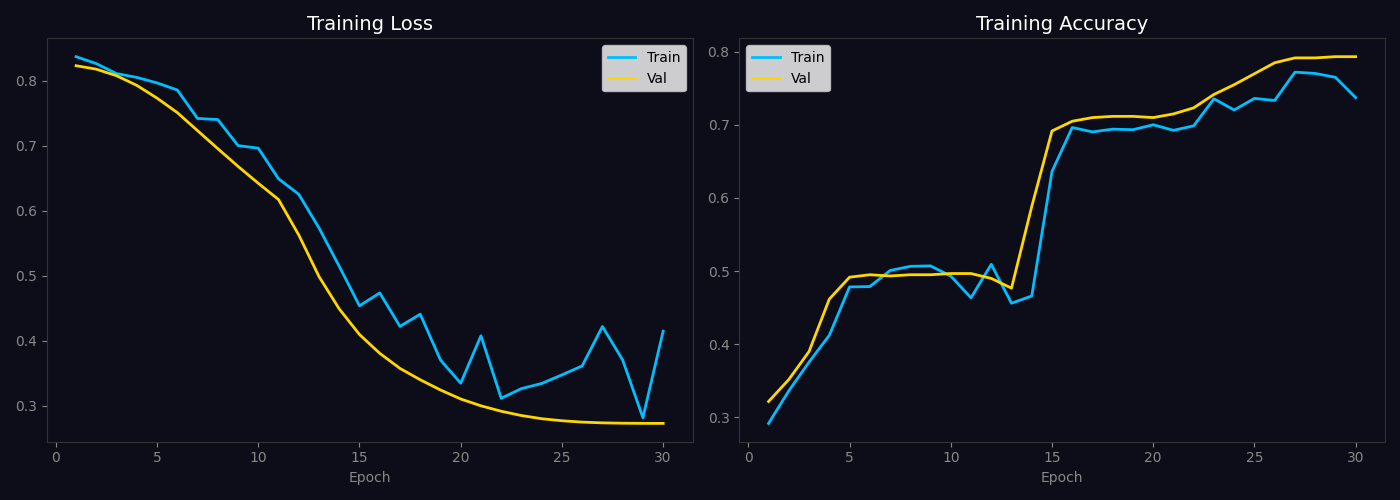
\includegraphics[width=\linewidth]{Figures/500param_classical_deadrelu_training_history.png}
  \caption{Classical ReLU control (C): the accuracy plateaus near 0.50 before
  partially escaping.}
  \label{fig:exp3_train_relu}
\end{subfigure}\hfill
\begin{subfigure}[t]{0.49\textwidth}
  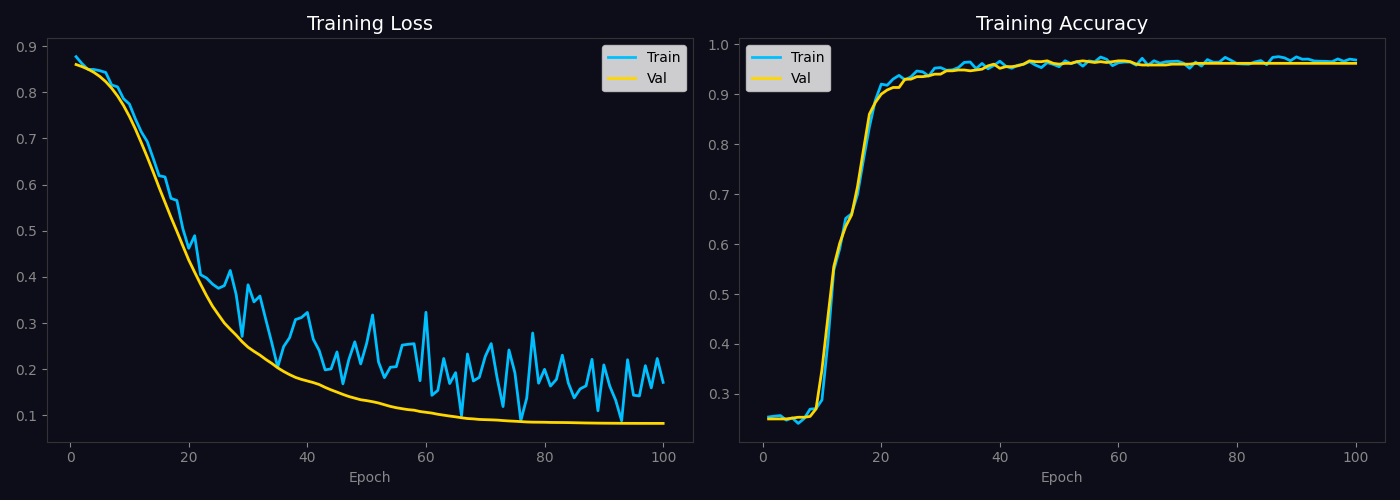
\includegraphics[width=\linewidth]{Figures/500param_classical_tanh_training_history.png}
  \caption{Classical Tanh control (D): clean, monotonic convergence.}
  \label{fig:exp3_train_tanh}
\end{subfigure}
\caption{Training history of the two 556-parameter classical controls. The only
difference between them is the inner activation function, which alone accounts for
the gap between 79\% and 96\% accuracy.}
\label{fig:exp3_training}
\end{figure*}

\subsubsection{Encoding ablation}

A separate set of variants probes whether the limitation lies in the number of
qubits or in how the features are loaded into them. Table~\ref{tab:exp3_encoding}
compares the learned linear encoding of Model~B against unsupervised PCA encodings.
A frozen PCA projection into the circuit caps accuracy near 76\% regardless of its
width, while the learned \texttt{Linear(128,4)} encoding into the same four qubits
reaches 96\%. PCA selects directions of maximum variance, which need not coincide
with directions of class separability, so it wastes the four encoding slots. A
learned linear layer instead selects discriminative directions end-to-end through
the loss. The bottleneck is therefore which four numbers enter the circuit, not the
four-qubit count, which identifies data encoding rather than circuit width as the
limiting factor for the quantum model.

\begin{table}[t]
\centering
\caption{Encoding ablation for the quantum head. All variants encode into four
qubits; only the projection feeding the circuit changes.}
\label{tab:exp3_encoding}
\setlength{\tabcolsep}{4pt}
\footnotesize
\begin{tabular}{lcc}
\toprule
Encoding into the VQC & Params & Acc. \\
\midrule
Frozen PCA(128,4)                  & $\sim$40  & $\sim$76\% \\
Frozen PCA(128,64) + Linear(64,4)  & $\sim$300 & $\sim$76\% \\
Learned Linear(128,4) (Model B)    & 556       & $\sim$96\% \\
\bottomrule
\end{tabular}
\end{table}

\subsubsection{Training dynamics and computational cost}

Beyond final accuracy we also examined convergence, stability and cost, since
parameter count alone is not a sufficient basis for comparison. The classical heads
are no slower to converge than the quantum head and are in fact faster, with the
dense head settling by about epoch 7 and the Tanh control by about epoch 20, against
about epoch 25 for the quantum head. All models show spiky training loss late in
training, which is a stochastic-gradient effect on small batches, but their
validation loss is smooth and monotonic, so the noise is in the optimiser rather
than in generalisation. The generalisation gap is essentially zero for the
556-parameter heads, as expected given the frozen backbone. The quantum head is far
more expensive to train, since each forward and backward pass is a statevector
simulation of the circuit that costs seconds per epoch on CPU, against milliseconds
for the classical heads, and on real quantum hardware it would additionally face
shot noise and decoherence.

\subsubsection{Summary of findings}

At matched parameter count the quantum head and the classical head reach the same
accuracy and the same per-class behaviour, so the result is quantum-classical parity
rather than a quantum advantage. The roughly $9\times$ saving of the 556-parameter
heads over the 5058-parameter dense head is real but is a property of the frozen
feature extractor, since the classical Tanh control obtains the same saving. The
single largest accuracy swing in the experiment, from 79\% to 96\% at identical
parameter count, came from the choice of activation function rather than from the
quantum or classical nature of the head, which supports the view that parameter
count alone is the wrong lens for these comparisons. We find no quantum advantage in
accuracy, parameter efficiency, convergence speed or training stability, and the
quantum model is considerably more costly to train. The methodological lesson is
that a variational quantum result should not be reported without a parameter-matched
classical control that uses a robust activation, because a width-limited ReLU
baseline can fail for reasons unrelated to capacity and create a false advantage.

\FloatBarrier
